\documentclass{anstrans}
%%%%%%%%%%%%%%%%%%%%%%%%%%%%%%%%%%%
\title{Validation of Isotopic Composition of Spent Nuclear Fuel output by Cyclus, a Fuel Cycle Simulator Code}
\author{Gwendolyn J. Chee, Gyutae Park, and Kathryn D. Huff}

\institute{
Dept. of Nuclear, Plasma and Radiological Engineering, University of Illinois at Urbana-Champaign \\
gchee2@illinois.edu
}

%%%% packages and definitions (optional)
\usepackage{graphicx} % allows inclusion of graphics
\usepackage{booktabs} % nice rules (thick lines) for tables
\usepackage{microtype} % improves typography for PDF
\usepackage{xspace}
\usepackage{tabularx}
\newcommand{\SN}{S$_N$}
\renewcommand{\vec}[1]{\bm{#1}} %vector is bold italic
\newcommand{\vd}{\bm{\cdot}} % slightly bold vector dot
\newcommand{\grad}{\vec{\nabla}} % gradient
\newcommand{\ud}{\mathop{}\!\mathrm{d}} % upright derivative symbol
\newcommand{\Cyclus}{\textsc{Cyclus}\xspace}%
\newcommand{\Cycamore}{\textsc{Cycamore}\xspace}%
\newcolumntype{c}{>{\hsize=.56\hsize}X}
\newcolumntype{b}{>{\hsize=.7\hsize}X}
\newcolumntype{s}{>{\hsize=.74\hsize}X}
\newcolumntype{f}{>{\hsize=.1\hsize}X}
\newcolumntype{a}{>{\hsize=.45\hsize}X}
\usepackage{titlesec}
\titleformat*{\subsection}{\normalfont}

\begin{document}
%%%%%%%%%%%%%%%%%%%%%%%%%%%%%%%%%%%%%%%%%%%%%%%%%%%%%%%%%%%%%%%%%%%%%%%%%%%%%%%%
\section{Introduction}
\Cyclus \cite{huff_fundamentals_2016}, a fuel cycle simulator, was used to run a simulation of the
United States' nuclear fuel cycle from 1967 up till 2013. \Cyclus spent nuclear fuel (SNF) data was compared to SNF data from the U.S Department of Energy (DOE) sponsored Unified Database (UDB) \cite{Peterson_UNF_2017}. The UDB provides comprehensive and consistent technical data on reactor sites and spent nuclear fuel (SNF) from 1967, the beginning of nuclear reactor operation in the United States, up to the year 2013. By comparing both sets of data, baseline comparison models between \Cyclus simulated results and real world metrics are established. 

%%%%%%%%%%%%%%%%%%%%%%%%%%%%%%%%%%%%%%%%%%%%%%%%%%%%%%%%%%%%%%%%%%%%%%%%%%%%%%%%
\section{Motivation}
The United States is considering various fuel cycles and geologic disposal options
\cite{DOE_strategy_2013}. The decisions made will be influenced by key criteria such as thermal load 
of waste packages and the thermal capacity of the selected geologic host media. Temperature information of thermal load of waste packages are dependent on the decay heat contribution from the isotopic composition of spent fuel. Accurate spent fuel isotopic composition data will in turn give accurate thermal load data. Therefore, to use \Cyclus to correctly model a nuclear waste repository, \Cyclus must first give isotopic composition and spent fuel mass that closely replicates reality. 

%%%%%%%%%%%%%%%%%%%%%%%%%%%%%%%%%%%%%%%%%%%%%%%%%%%%%%%%%%%%%%%%%%%%%%%%%%%%%%%%
\section{Methodology}
\subsection{\textit{Generating \Cyclus Simulation and Analysis}}
Published data of the 112 commerical nuclear reactors that have operated since 1967 in the United States was used to create a \Cyclus simulation of the United States Nuclear Fuel Cycle. There were 2 main types of data required to create the simulation: fresh and spent fuel recipes, and reactor deployment data. The recipes are from the vision datebase \cite{vision}. The reactor deployment data was obtained from the Power Reactor Information System's (PRIS) reactor database \cite{IAEA_PRIS_2017}.

Jinja2 \cite{Ronacher_Jinja2_2018}, a Python templating language, was used in Python to render the previously mentioned data into an input file that can be accepted by \Cyclus. The output file produced by \Cyclus was analyzed using Python. 

\subsection{\textit{UDB Data Analysis}}
The UDB data contains SNF information from 1967 up till 2013. The dataset included discharged fuel assembly data from each reactor with specific isotopic concentrations and decay heat for each assembly including the date it was discharged \cite{Peterson_UNF_2017}. The data was imported into Python and processed to be compared with \Cyclus data. 
%%%%%%%%%%%%%%%%%%%%%%%%%%%%%%%%%%%%%%%%%%%%%%%%%%%%%%%%%%%%%%%%%%%%%%%%%%%%%%%%
\section{Results and Analysis}
The primary outcome of this validation is to provide comparisons between \Cyclus and UDB data for spent fuel mass and major isotopic contributions to the total spent fuel mass. 

\subsection{\textit{Cumulative Total Spent Fuel Mass Comparison}}
Figure \ref{fig:total_original} shows the cumulative spent fuel mass for both \Cyclus and UDB data from 1967 to 2013. The total spent fuel mass produced by \Cyclus is larger than UDB data pre-2000. Post-2000, the \Cyclus and UDB total spent fuel mass data diverge, with UDB being larger. The discrepancies can be attributed to rigidity of \Cyclus simulation input with respect to cycle and refuel time. In \Cyclus, the user specifies constant month integer refuel and cycle times for each reactor. In reality, the cycle and refuel times are varied throughout each reactor's lifetime and may not fall in exactly month length-ed times. In the \Cyclus simulation, the cycle time and refuel time were assumed to be constants of 18 and 1 month respectively.   

\begin{figure}[ht] % replace 't' with 'b' to force it to be on the bottom
	\centering
	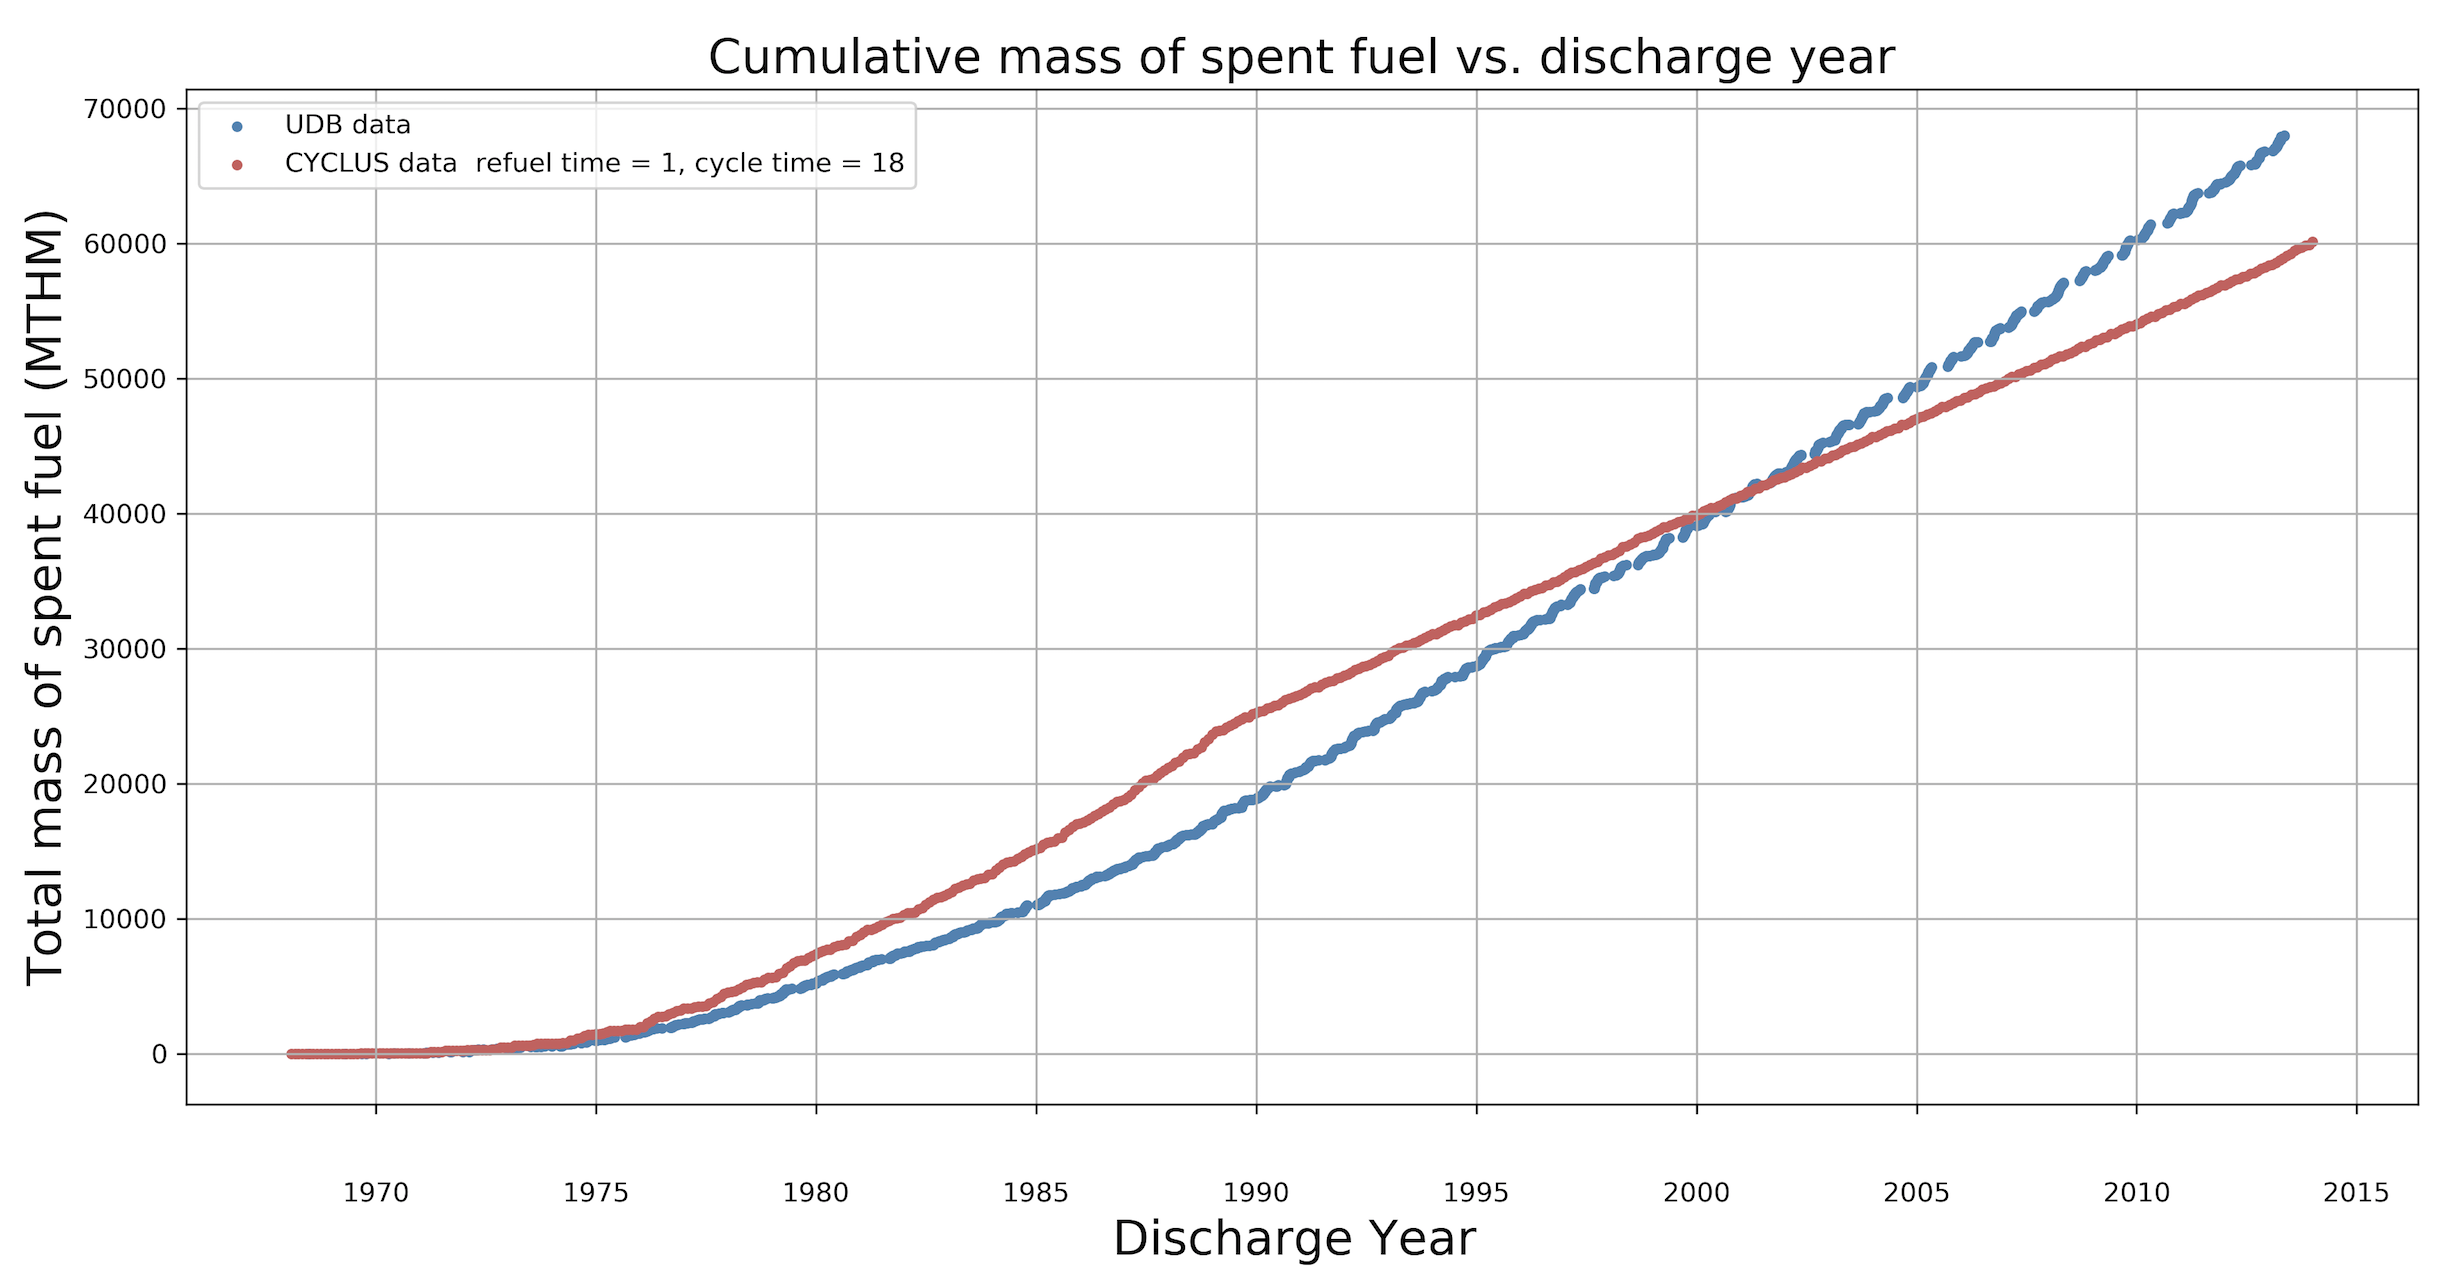
\includegraphics[width=0.48\textwidth]{total_cumulative_mass_spent_fuel_original}
	\caption{Total cumulative spent fuel mass against discharge time for \Cyclus and UDB data from 1967 up to 2013}
	\label{fig:total_original}
\end{figure}

It was reported by the Nuclear Energy Institute (NEI) that there has been significant variance in the refueling period for reactors in the United States. The average refuelling time in 1990 was 104 days, and generally decreased to an average refuelling time of 35 days in 2017 \cite{nei}.

The \Cyclus spent fuel mass data being larger than UDB data pre-2000 can be attributed to the assumption that refueling time is always 1 month. Figure \ref{fig:total_refueltime} includes plots of total spent fuel mass from \Cyclus simulations where refuel time is increased. A larger refuel time brings the total spent fuel mass from \Cyclus simulations closer to the UDB data pre-2000. 

\begin{figure}[ht] % replace 't' with 'b' to force it to be on the bottom
	\centering
	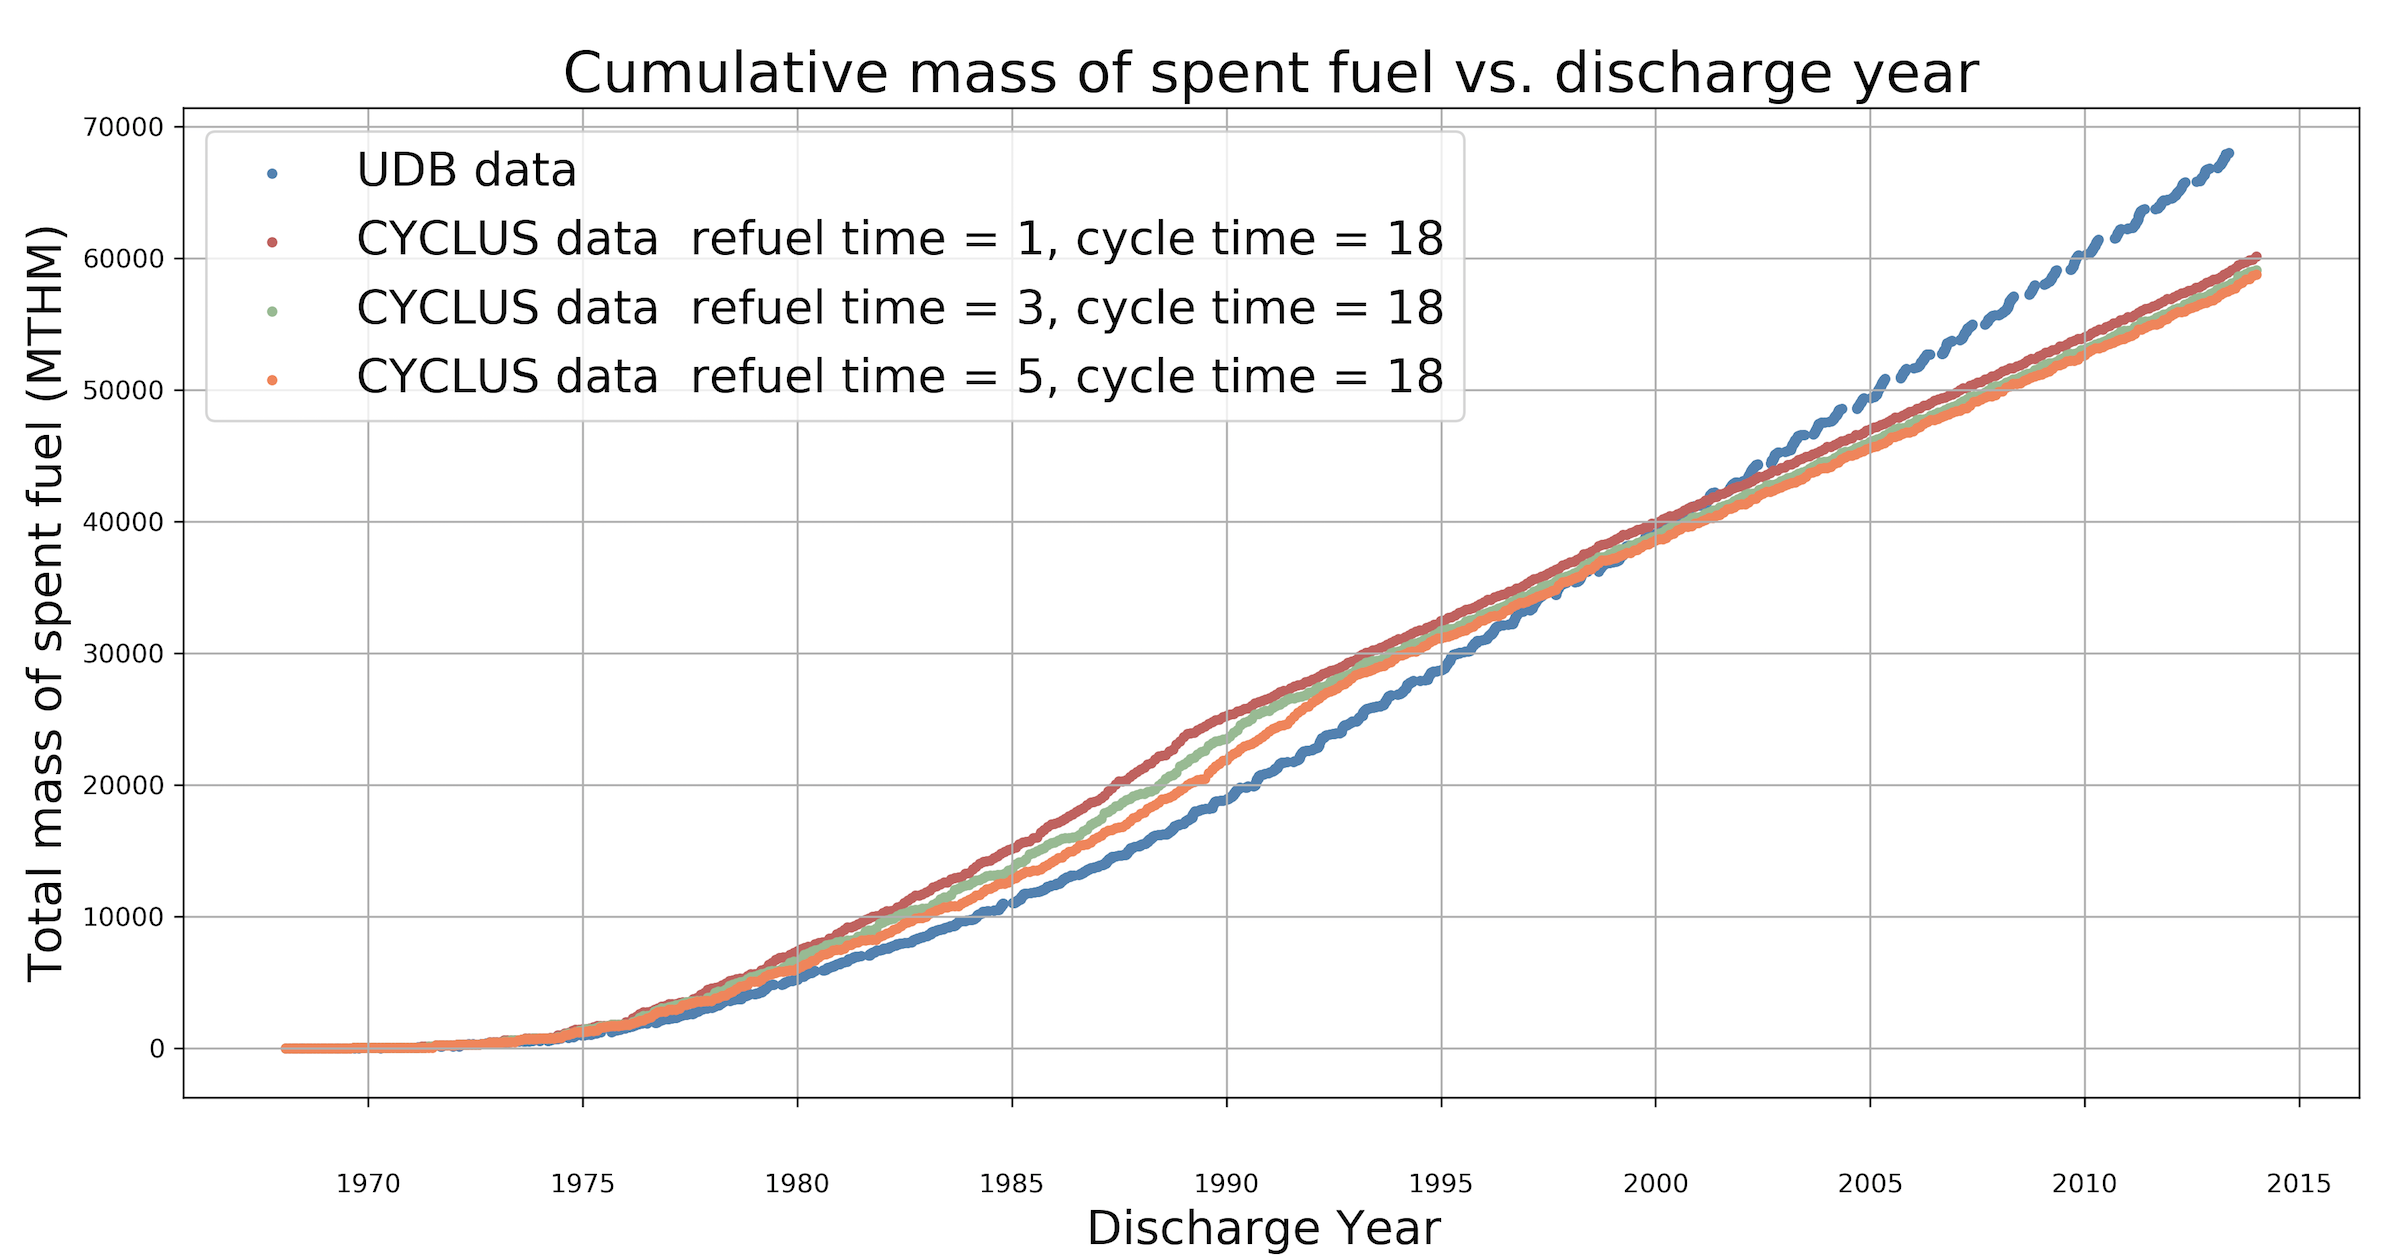
\includegraphics[width=0.48\textwidth]{total_cumulative_mass_spent_fuel_refueltime}
	\caption{Total cumulative spent fuel mass against discharge time for \Cyclus and UDB data from 1967 up to 2013 for varying refuel time}
	\label{fig:total_refueltime}
\end{figure} 

 IAEA reported that the average cycle time has an increasing trend. Average cycle time was 400 days in 1990 and 500 days in 2004 \cite{IAEA}. There is an upward trend of cycle time and downward trend of refuel time where cycle time increases faster than refuel time. 
The larger amount of UDB spent fuel mass compared to \Cyclus data post-2000 could be attributed to the cycle length of reality being shorter than the 19 month length of \Cyclus simulations. 

Figure \ref{fig:total_cycletime} includes plots of total spent fuel mass from \Cyclus simulations where cycle time is varied. A shorter cycle time brings the total spent fuel mass from \Cyclus simulations closer to the UDB data post-2000. 

\begin{figure}[ht] % replace 't' with 'b' to force it to be on the bottom
	\centering
	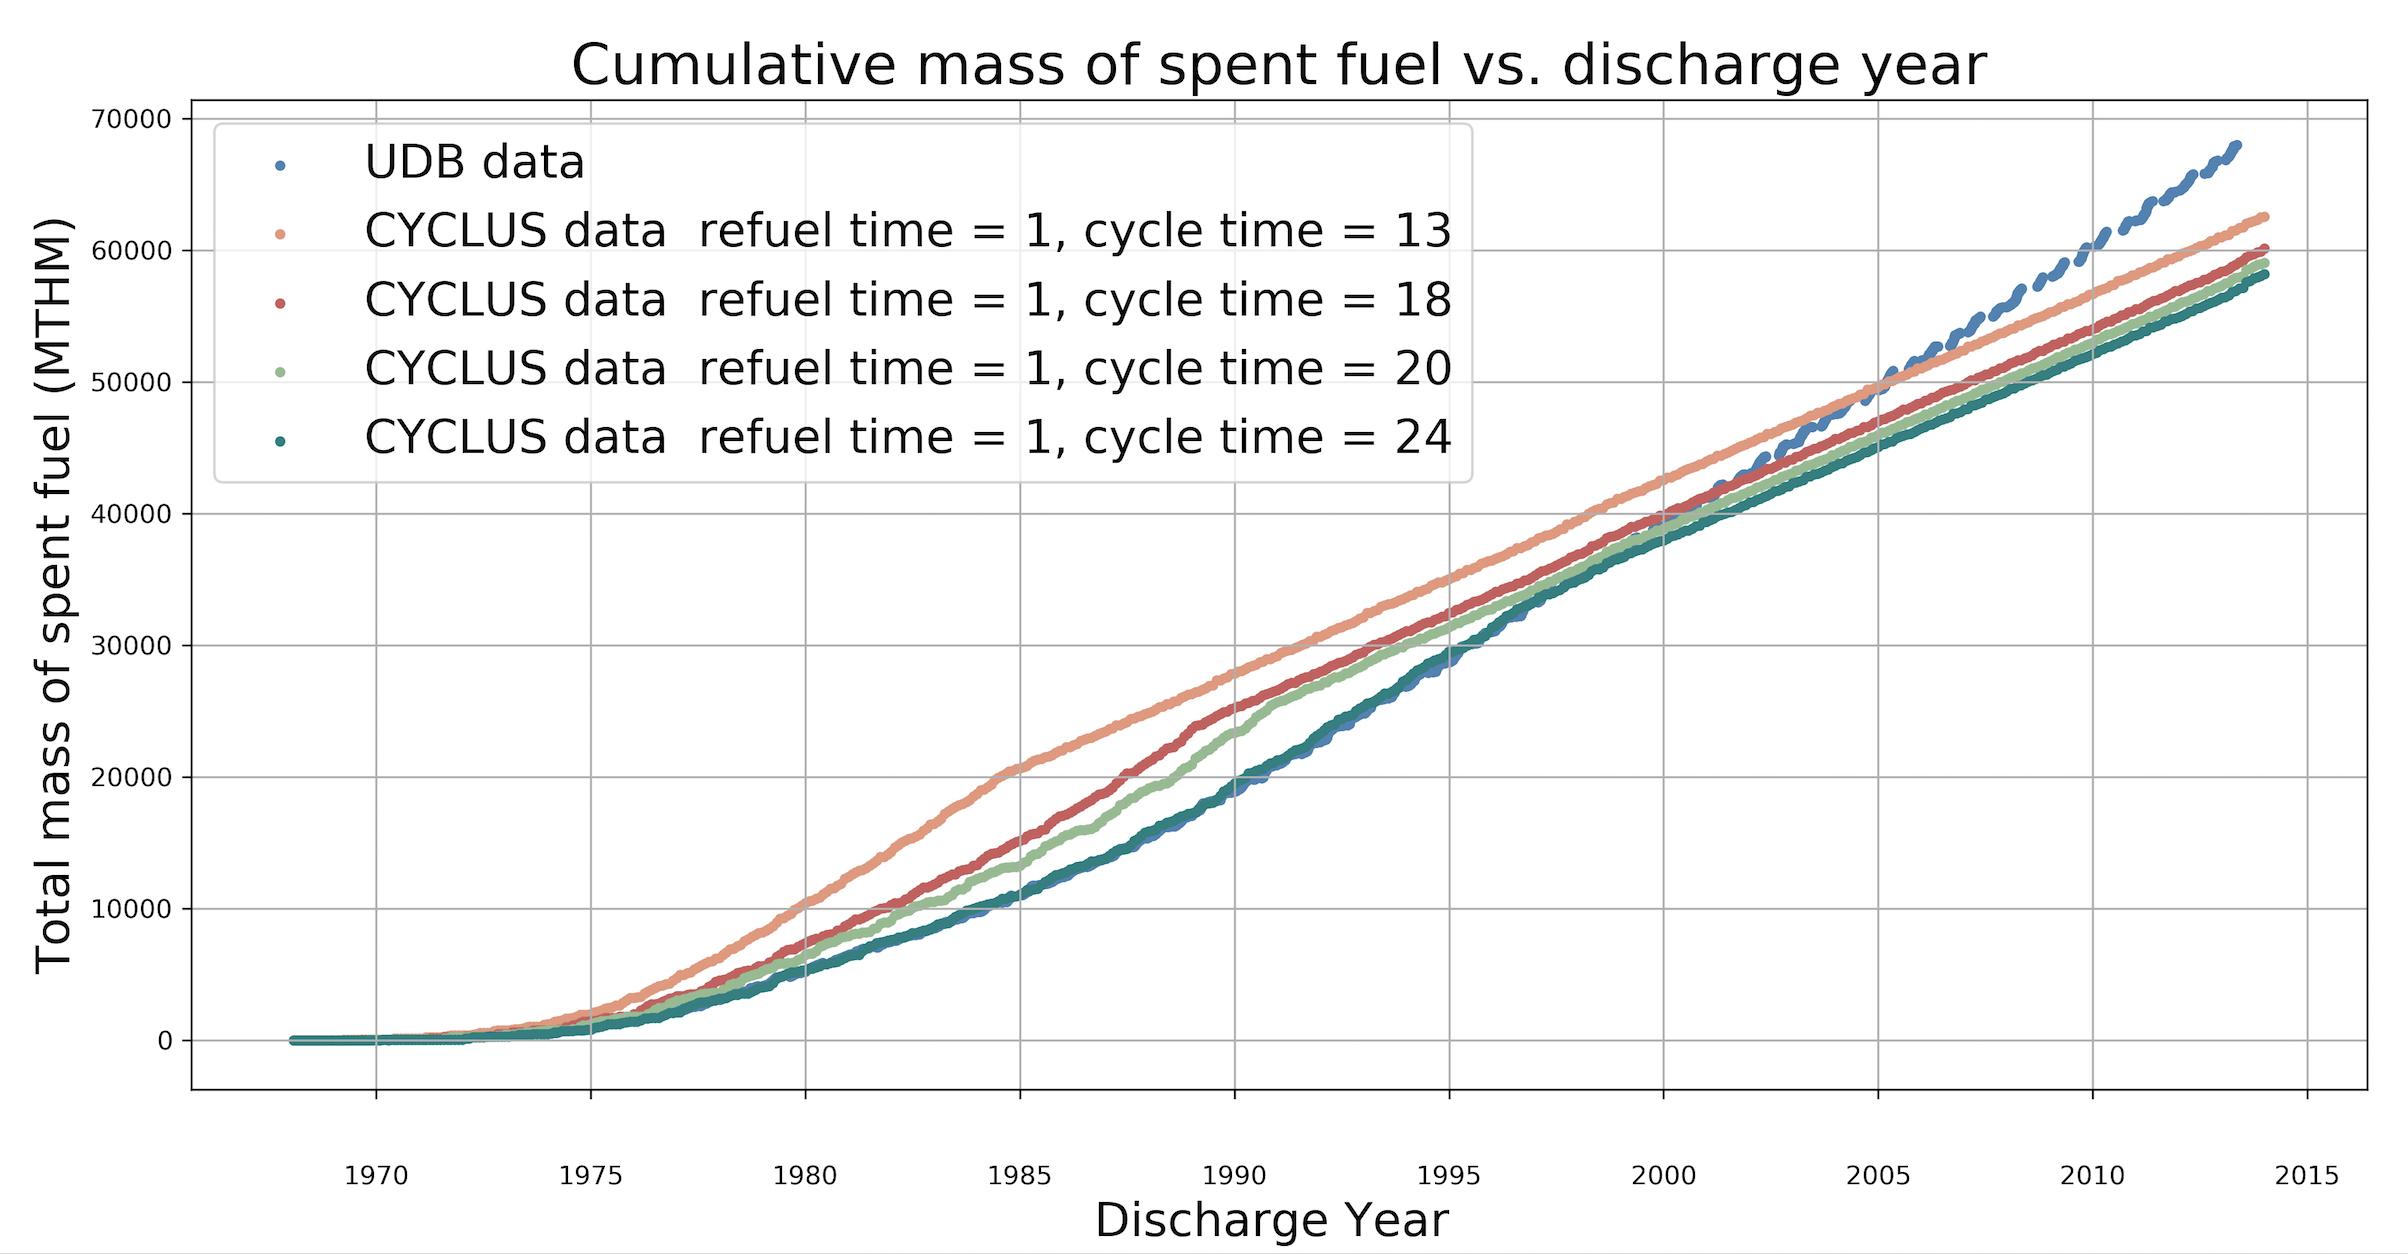
\includegraphics[width=0.48\textwidth]{total_cumulative_mass_spent_fuel_cycletime}
	\caption{Total cumulative spent fuel mass against discharge time for \Cyclus and UDB data from 1967 to 2013 for varying cycle time}
	\label{fig:total_cycletime}
\end{figure} 

\subsection{\textit{Major Isotopic Composition of  Spent Fuel Mass Comparison}}
The isotopes that contribute the most to the total mass of the spent fuel in order of significance are: U-238, U-235, Pu-239, U-236 and Pu-240.   

Figure \ref{fig:total_u238}, \ref{fig:total_u235} and \ref{fig:total_pu240} shows the cumulative spent fuel mass for U-238, U-235 and pPu-239 isotope for both \Cyclus and UDB data from 1967 to 2013.
They follow the same trend as figure \ref{fig:total_original} and the same explanations can be used to explain the differences in values. 

\begin{figure}[ht] % replace 't' with 'b' to force it to be on the bottom
	\centering
	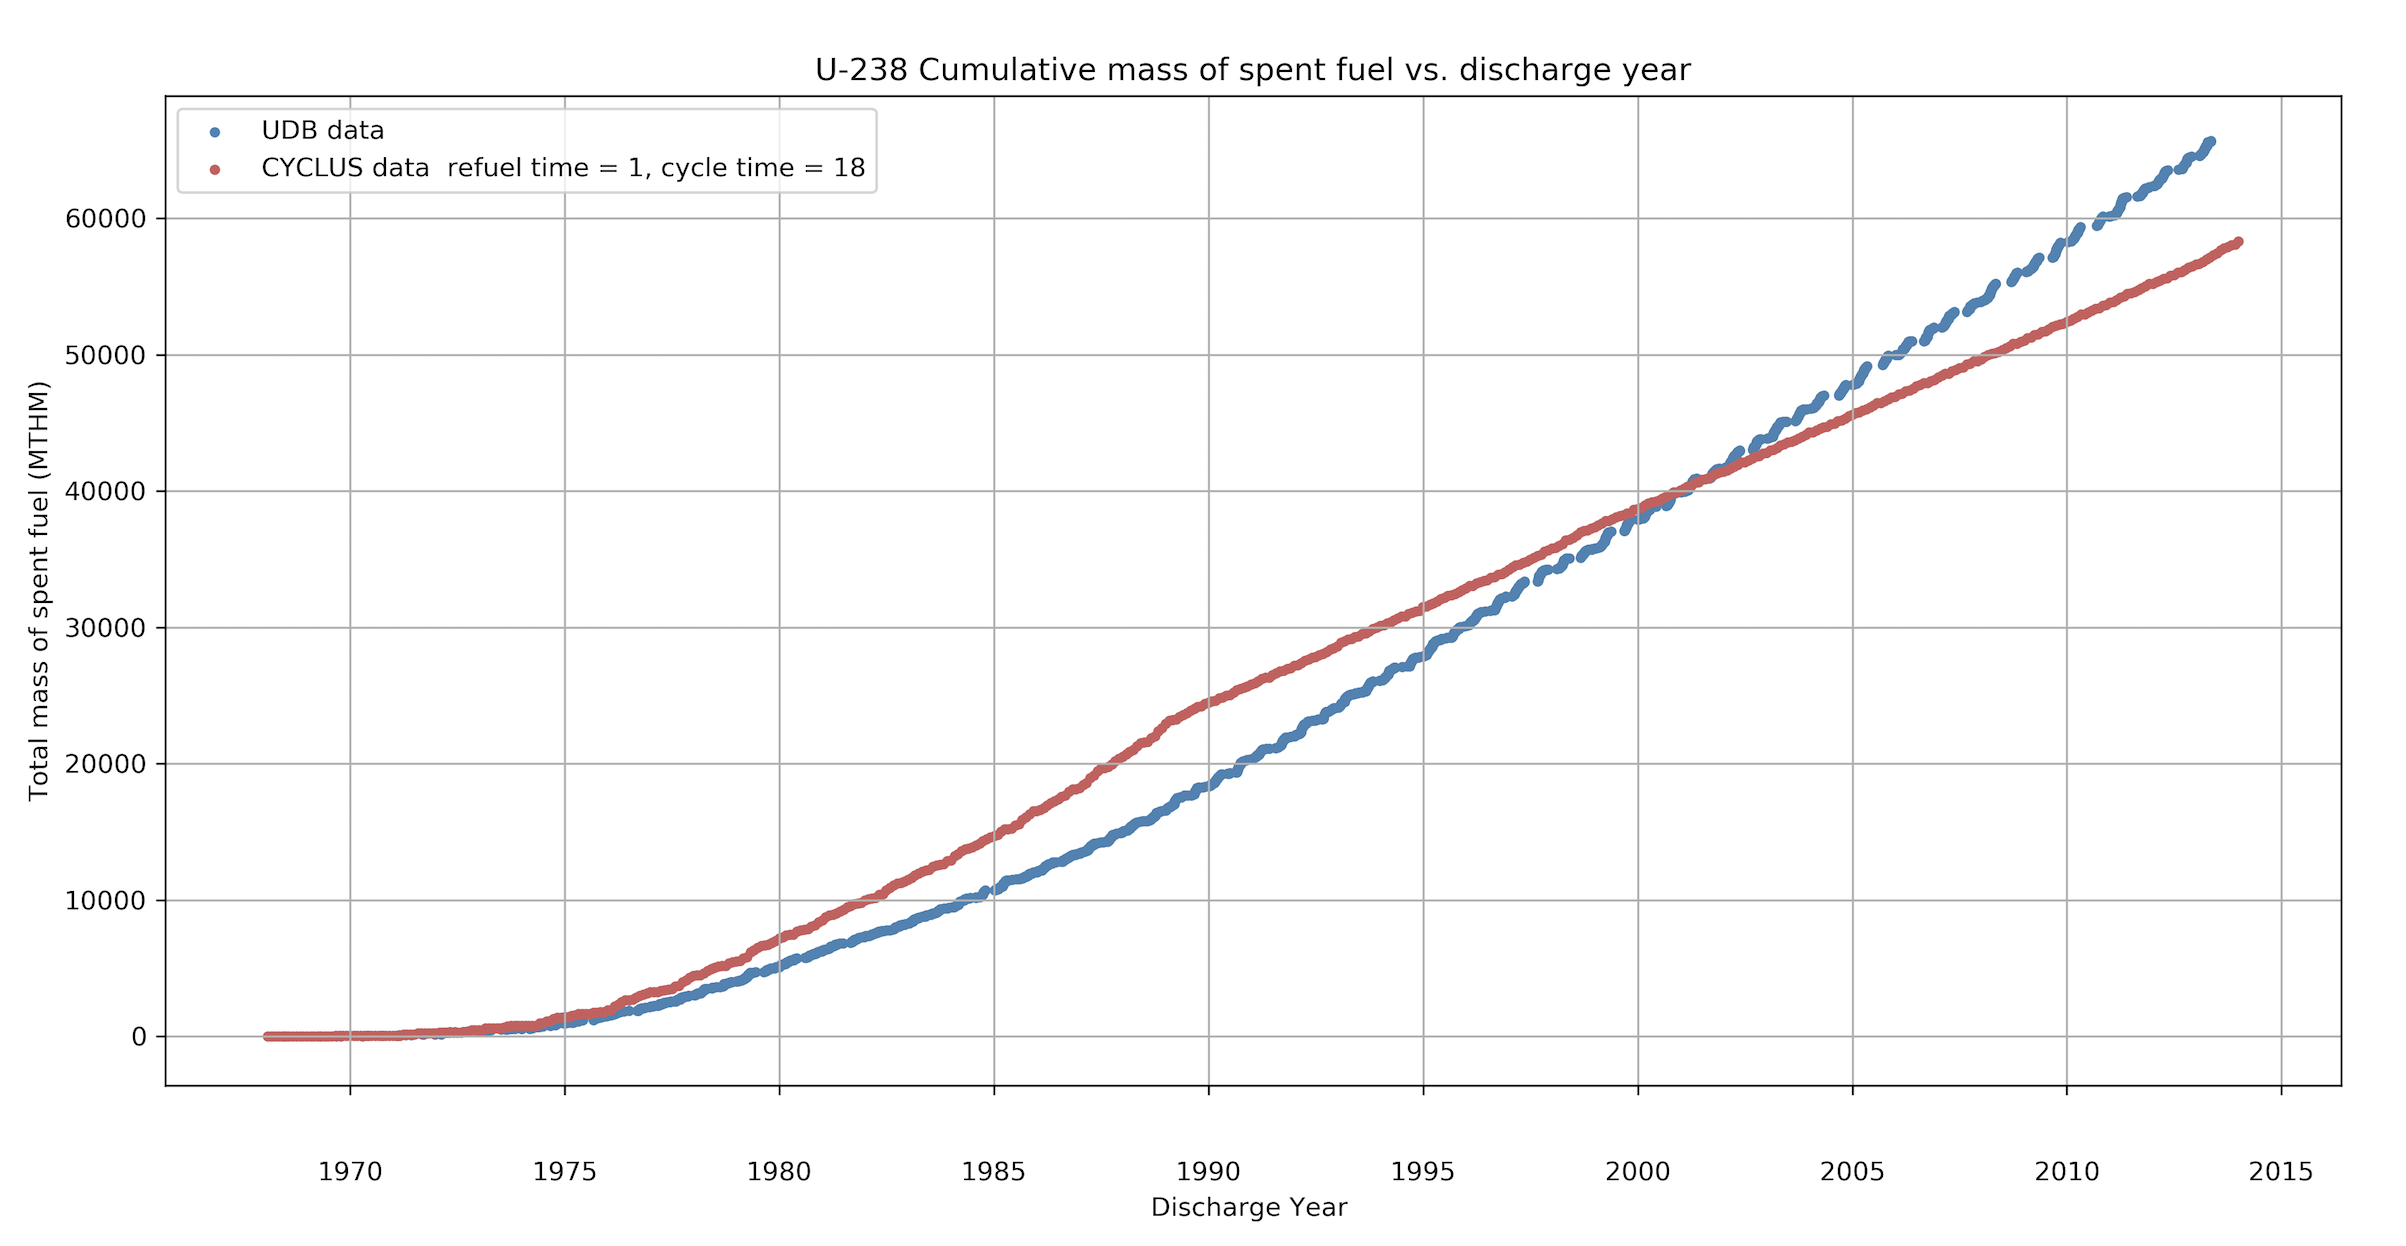
\includegraphics[width=0.48\textwidth]{U-238_cumulative_mass_spent_fuel_original}
	\caption{Total cumulative spent fuel mass of U-238 isotope against discharge time for \Cyclus and UDB data from 1967 up to 2013}
	\label{fig:total_u238}
\end{figure}

\begin{figure}[ht] % replace 't' with 'b' to force it to be on the bottom
	\centering
	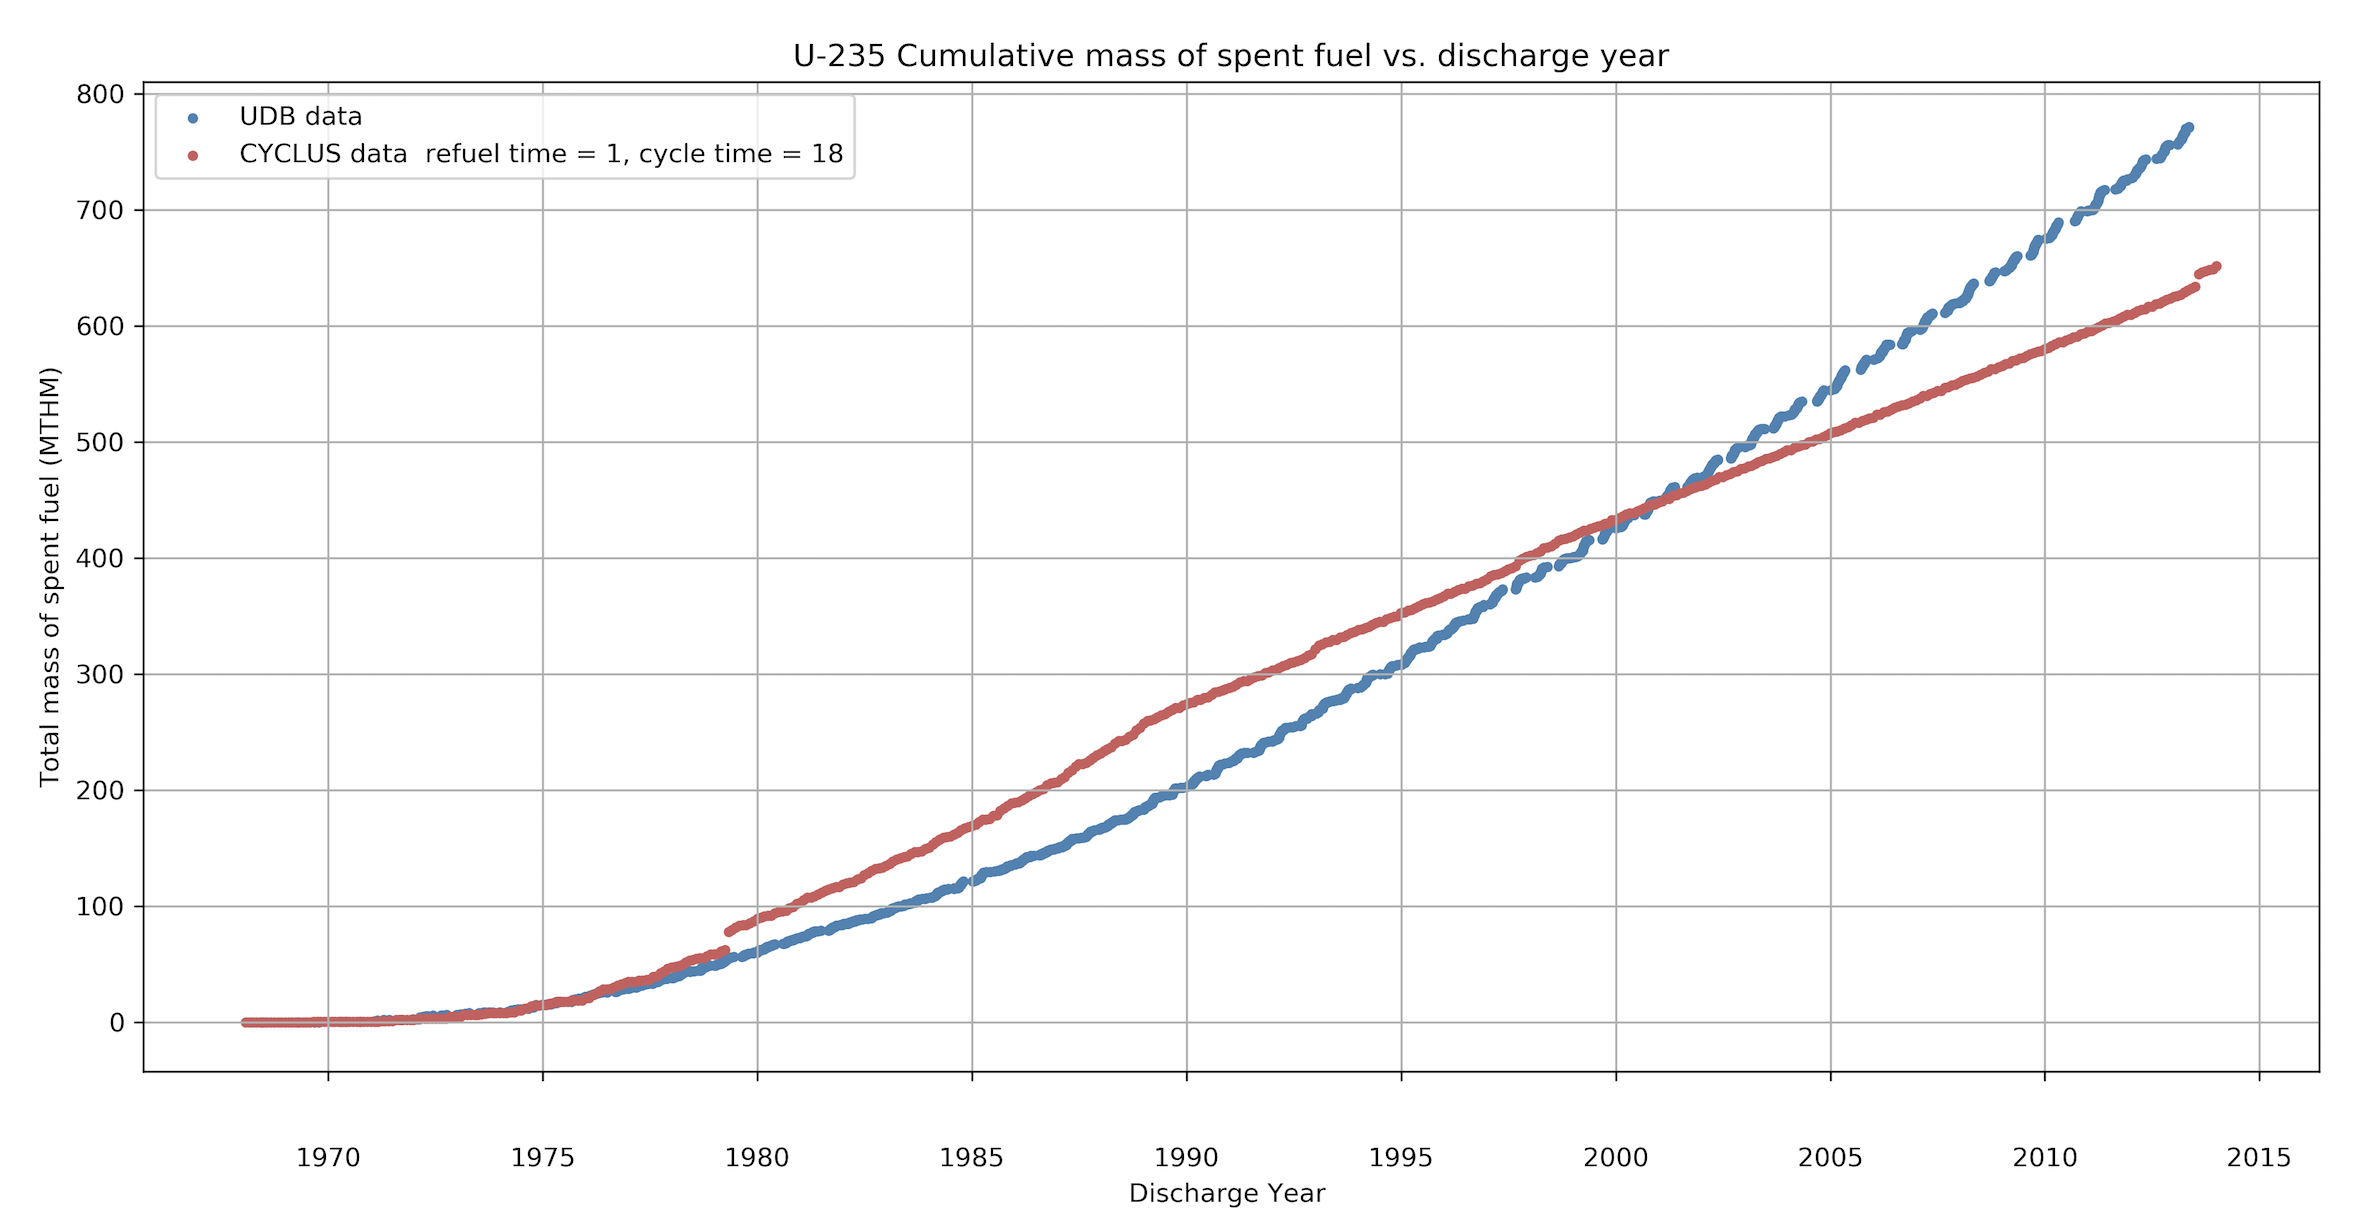
\includegraphics[width=0.48\textwidth]{U-235_cumulative_mass_spent_fuel_original}
	\caption{Total cumulative spent fuel mass of U-235 isotope against discharge time for \Cyclus and UDB data from 1967 up to 2013}
	\label{fig:total_u235}
\end{figure}

\begin{figure}[hb] % replace 't' with 'b' to force it to be on the bottom
	\centering
	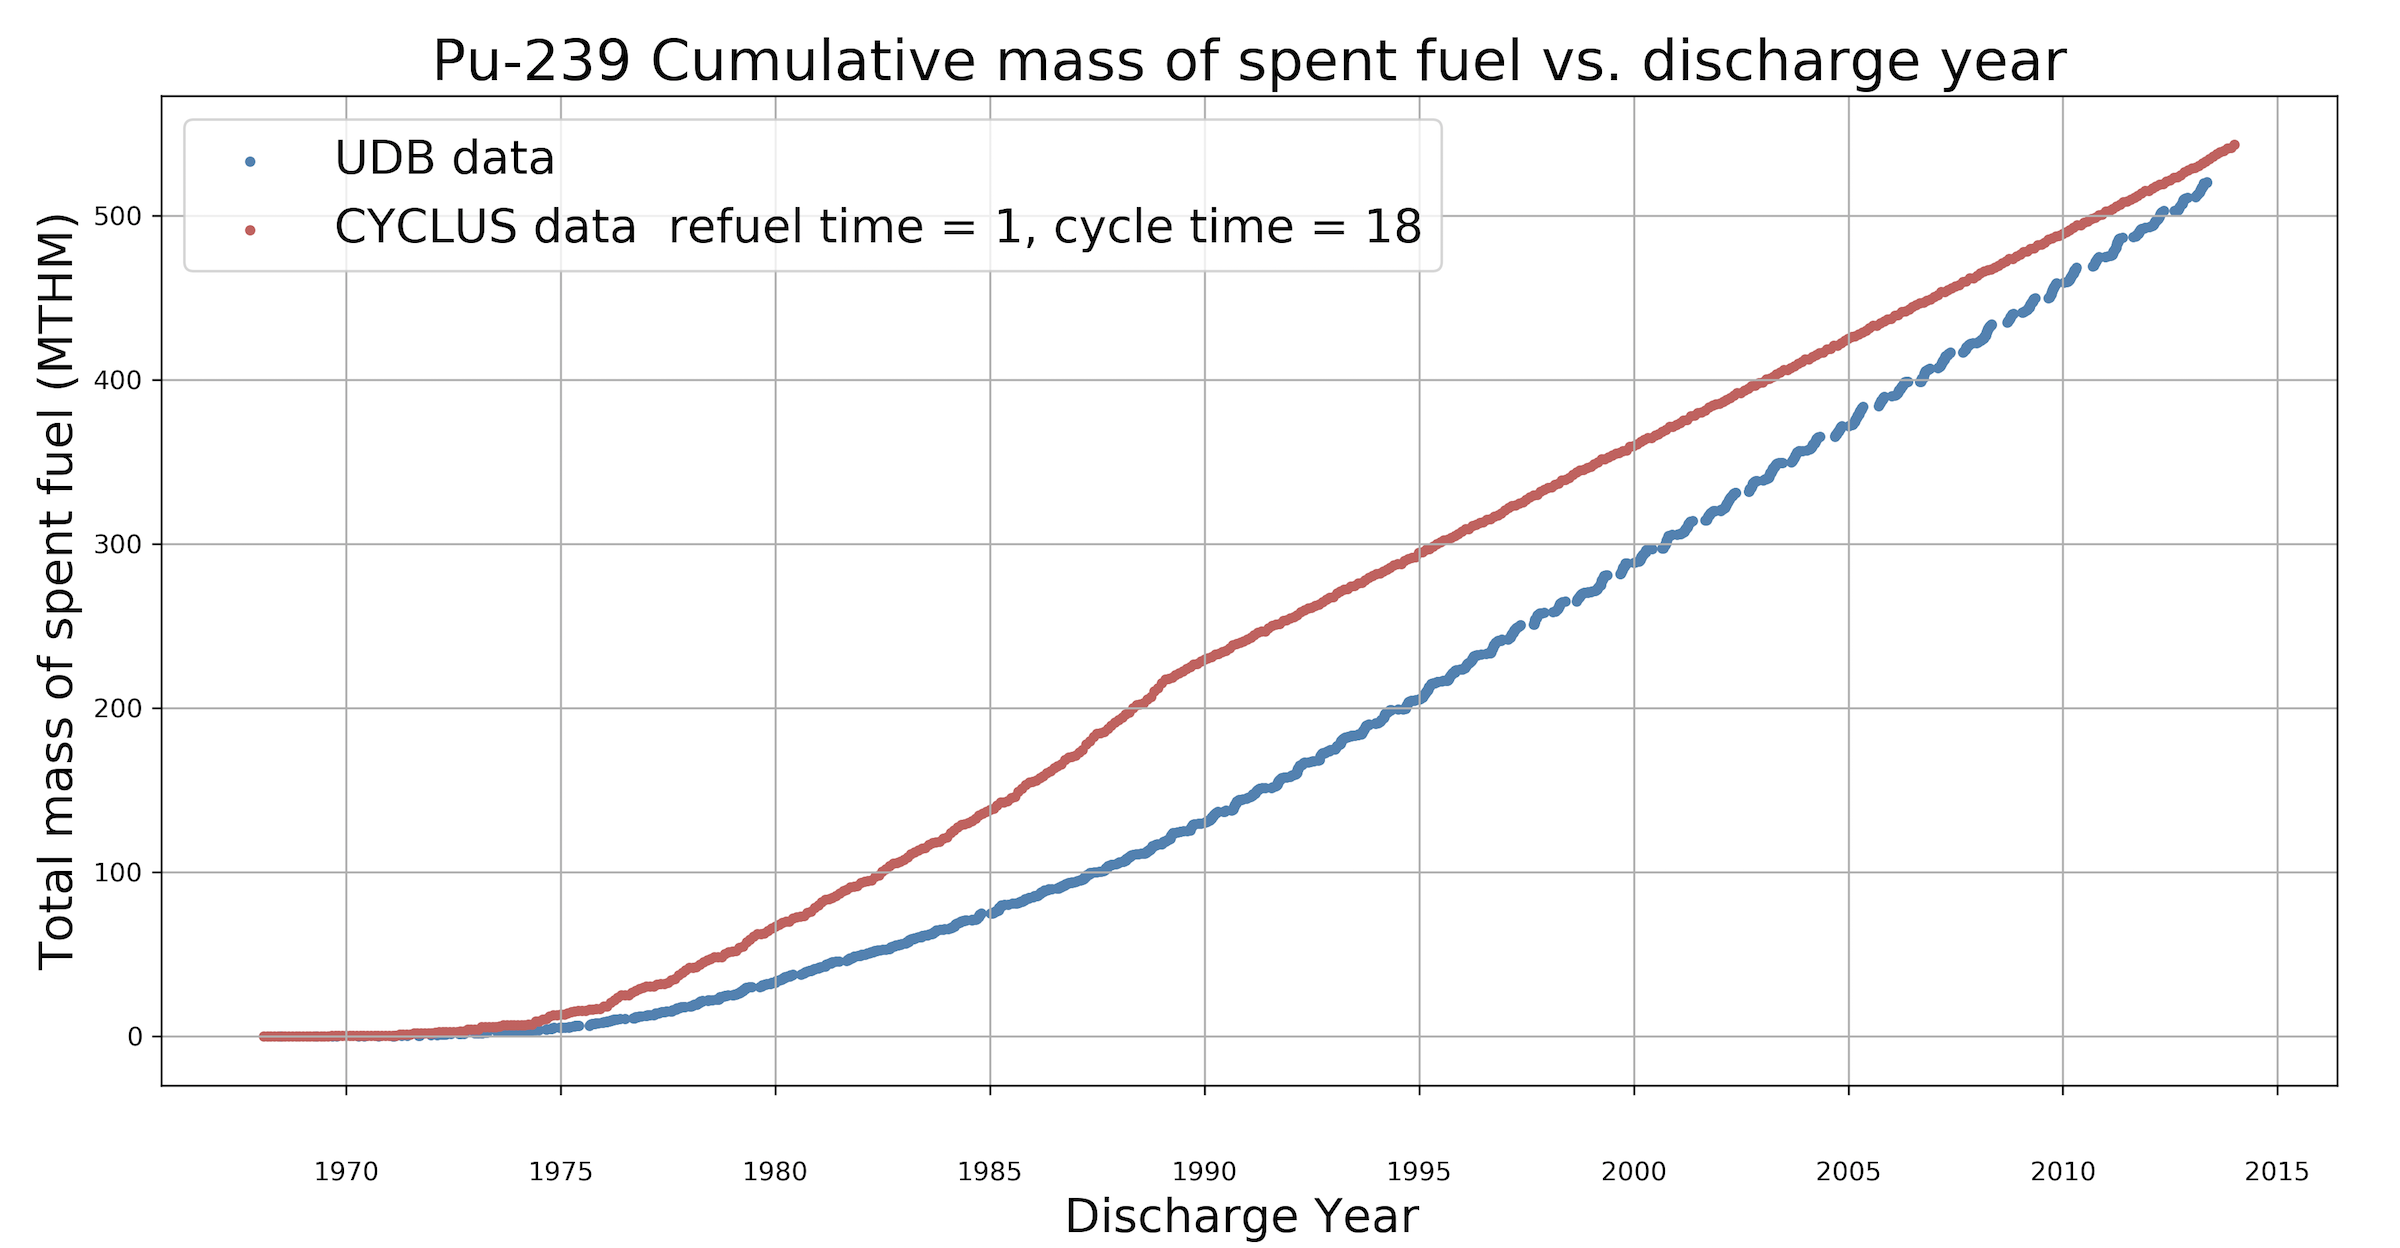
\includegraphics[width=0.48\textwidth]{Pu-239_cumulative_mass_spent_fuel_original}
	\caption{Total cumulative spent fuel mass of Pu-239 isotope against discharge time for \Cyclus and UDB data from 1967 up to 2013}
	\label{fig:total_pu239}
\end{figure}
%%%%%%%%%%%%%%%%%%%%%%%%%%%%%%%%%%%%%%%%%%%%%%%%%%%%%%%%%%%%%%%%%%%%%%%%%%%%%%%%
\pagebreak
\section{Conclusions}
Further work to improve \Cyclus simulations so that it can more closely reflect reality is to give the reactor archetype capability to accept varying cycle and refuel times. Thus, by looking at the historic United States reactor operating data, a \Cyclus simulation can be made to replicate their cycle and refuel times even more closely. 

Therefore, with more accurate spent fuel mass and isotopic compositions, the simulations for thermal loading of a waste repository will be more accurate. 
%%%%%%%%%%%%%%%%%%%%%%%%%%%%%%%%%%%%%%%%%%%%%%%%%%%%%%%%%%%%%%%%%%%%%%%%%%%%%%%%
\section{Acknowledgments}
This research is being performed using funding received from the DOE Office of Nuclear Energy's
Nuclear Energy University Program (Project 16-10512) "Demand-Driven Cycamore Archetypes". 

%%%%%%%%%%%%%%%%%%%%%%%%%%%%%%%%%%%%%%%%%%%%%%%%%%%%%%%%%%%%%%%%%%%%%%%%%%%%%%%%
\bibliographystyle{ans}
\bibliography{bibliography}
\end{document}

